\clearpage
\section{Radian As A Unit Of Measurement}
Now to discuss what exactly a radian is.

The measurement is derived from arc lengths starting from the positive $x$-direction of a circle with a radius of $r = 1$, also known as the \textbf{unit circle} ("unit" signifies the $1$ unit radius of the circle).

Try thinking about it this way:

Place a circle with radius $1$ at to origin, such that it's center is at $(0,0)$. That should look something like the figure below.
\begin{center}
    \begin{minipage}[c]{0.33\linewidth}
        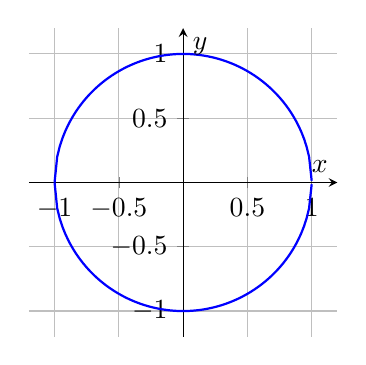
\begin{tikzpicture}
            \begin{axis}[
                axis lines = middle,
                xlabel = $x$, ylabel = {$y$},
                xmin = -1.2, xmax = 1.2,
                ymin = -1.2, ymax = 1.2,
                xtick distance={0.5}, ytick distance={0.5},
                width = 5.5cm,
                height = 5.5cm,
                grid = both,
                legend pos = south east,
            ]
                \addplot[blue, thick, domain=-1:1, samples=100] {sqrt(1 - x^2)};
                \addplot[blue, thick, domain=-1:1, samples=100] {-1 * sqrt(1 - x^2)};
            \end{axis}
        \end{tikzpicture}
    \end{minipage}
    \begin{minipage}[c]{0.66\linewidth}
        The equation for the circumference, $C$, of a circle is
        \[
            C = 2\pi r \text{.}
        \]
        Because we're working with a circle that has a radius of $r = 1$, we have:
        \[
            C = 2\pi \text{.}
        \]
    \end{minipage}
\end{center}
This means, if you start from the positive $x$ direction, move counter-clockwise around the entire circle, and eventually return to the positive $x$ direction, you'll have traveled $2\pi$ radians.

Now, suppose you wanted to draw a line that starts from the center of the circle at $(0,0)$ and ends at the perimeter of the circle. 

For the purposes of understanding radians, assume the line you drew starts at $(0,0)$ and ends at $(0,1)$ (that's straight up from the origin). We'll call this line $L$. 

The angle, in radians, formed by the line $L$ and the positive $x$-axis is the length of the arc that starts from the positive $x$-axis to the point where $L$ touches the circle.
\begin{center}
    \begin{minipage}[c]{0.33\linewidth}
        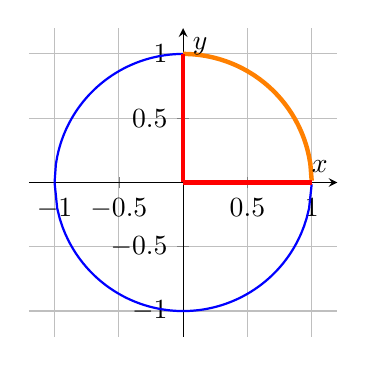
\begin{tikzpicture}
            \begin{axis}[
                axis lines = middle,
                xlabel = $x$, ylabel = {$y$},
                xmin = -1.2, xmax = 1.2,
                ymin = -1.2, ymax = 1.2,
                xtick distance={0.5}, ytick distance={0.5},
                width = 5.5cm,
                height = 5.5cm,
                grid = both,
                legend pos = south east,
            ]
                \addplot[blue, thick, domain=-1:0, samples=100] {sqrt(1 - x^2)};
                \addplot[blue, thick, domain=-1:1, samples=100] {-1 * sqrt(1 - x^2)};
                % %
                \addplot[orange, ultra thick, domain=0:1, samples=100] {sqrt(1 - x^2)}; %Arc length
                \addplot[red, ultra thick, domain=0:1, samples=10] {0};
                \draw[red, ultra thick] (0,0) -- (0,1); %Line from origin to (0,1)
            \end{axis}
        \end{tikzpicture}
    \end{minipage}
    \begin{minipage}[c]{0.66\linewidth}
        Denoted in red are:
        \begin{itemize}
            \item The vertical line, $L$, drawn from the origin.
            \item The positive $x$-axis that is within the circle.
        \end{itemize}
        Denoted in orange is the arc created from the positive $x$-axis to where the vertical line touches the circle.
    \end{minipage}
\end{center}
Notice that this arc is one-fourth of the circumference of the circle.

We've already established that the entire circumference of the circle is $2\pi$. Therefore, we can say that the length of the orange arc is $\frac{\pi}{2}$.

With that, we've now found that the angle formed by the two red lines creates an angle that is $\frac{\pi}{2}$ radians.

Rest assured that you \textbf{do not} have to find the length of an arc on the unit circle every time you want to find angles in radians. In fact, for the foreseeable future, you don't have to find any angles at all.

The example above only serves to demonstrate what exactly a measurement in radians is supposed to mean.
\clearpage
\subsection{Why a Radius of 1?}
Using a radius of $1$ makes the math so much easier. It:
\begin{enumerate}
    \item Removes the radius from the circumference equation $C = 2\pi$.
    \item Exponentially simplifies the trigonometric identities you'll learn later in this part.
    
    For example, the Pythagorean Identity with $r = 1$ is $\sin^2(\theta) + \cos^2(\theta) = 1$ (beautiful). If you used $r = 0.5$, you'd have $\sin^2(\theta) + \cos^2(\theta) = 0.25$ (that's ugly). With $r = 1$, you get $1^2 = 1$. With $r = 0.5$, you get $0.5^2 = 0.25$.
    \item It simplifies differentiation and integration (topics you'll be introduced to in Calculus I and expanded upon in Calculus II and III).
    
    For example, if you used $r = 2$ with Trigonometric Substitution (covered in Calculus II), you could no longer easily use the following:
    \begin{itemize}
        \item For $\sqrt{a^2 - x^2}$, use $x = a\sin(\theta)$
        \item For $\sqrt{a^2 + x^2}$, use $x = a\tan(\theta)$
        \item For $\sqrt{x^2 - a^2}$, use $x = a\sec(\theta)$
    \end{itemize}
    The above are built on the idea that $r = 1$. Changing that would require you, and the entire mathemematics community, to rethink how they work.
\end{enumerate}
These are only three of the \textbf{many} things that rely on $r = 1$, some of which go beyond what \textit{I} know. Long story short, stick with $r = 1$. It's the sweet spot that makes everything much, \textbf{much} easier.